\documentclass{beamer}
\usetheme{Boadilla}
\usepackage{hyperref}
\usepackage{graphicx}
\usepackage{fancyvrb}
\usepackage{multicol}
\usepackage{subfig}
\usepackage[
    backend=biber, 
    natbib=true,
    style=numeric,
    sorting=none,
    style=verbose-ibid,
]{biblatex}
\addbibresource{citations.bib}
\usepackage{pgfpages}
\usepackage{xcolor}
\definecolor{ao(english)}{rgb}{0.0, 0.5, 0.0}
\definecolor{burgundy}{rgb}{0.5, 0.0, 0.13}
%\setbeameroption{show notes}
\setbeameroption{show notes on second screen=right}
%\setbeameroption{hide notes}

\title{Gabor's 1946 Theory of Communication}
\author{Sevag Hanssian}
\institute{MUMT 622, Winter 2021}
\setbeamertemplate{navigation symbols}{}

\begin{document}

\begin{frame}
\maketitle
\end{frame}

\begin{frame}
	\frametitle{Significance}
	Outcomes of Gabor's 1946 paper, ``Theory of Communication''\footfullcite{gabor1946}:
	\vspace{0.5em}
	\begin{enumerate}
		\item
			First introduction of the time-frequency uncertainty principle, leading to interest in wavelets\footfullcite{homage1}
		\item
			First use of the STFT for analysis of speech\footfullcite{textbook1}
			\begin{quote}
			The earliest application of a local Fourier analysis was by Dennis Gabor to the analysis of speech
			\end{quote}
		\item
			\vspace{-0.35em}
			Signal representation with Gabor elementary functions (Gaussian-modulated sinusoids) to minimize time-frequency uncertainty
	\end{enumerate}
\end{frame}

\begin{frame}
	\frametitle{Heisenberg's Uncertainty Principle}
	Heisenberg's uncertainty principle in quantum physics\footfullcite{hallm}:
	    \[ \sigma_{x}\sigma_{p} \ge \frac{h}{4\pi} \]
	    Heisenberg, 1927:
	    \begin{quote}
		    the more precisely the position [of an electron] is determined, the less precisely the momentum is known, and conversely
	    \end{quote}
\end{frame}

\note{
	\begin{itemize}
		\item
			in the world of quantum physics this is a core of the Copenhagen school, which Einstein disagreed with. this seems to be a fundamental limitation of the universe (as far as we know it)
	\end{itemize}
}

\begin{frame}
	\frametitle{Gabor's Uncertainty Principle}
	Gabor's time-frequency uncertainty:
	    \[ \sigma_{t}\sigma_{f} \ge \frac{1}{4\pi},\qquad\Delta t\Delta f \ge 1 \]
	    Gabor, 1946:\footfullcite{gabor1946}
	    \begin{quote}
		    although we can carry out the analysis with any degree of accuracy in the time direction or frequency direction, we cannot carry it out simultaneously in both beyond a certain limit
	    \end{quote}
\end{frame}

\note{
	\begin{itemize}
		\item
			Gabor says delta f and delta t are the uncertainties inherent in the definition of the epoch t and frequency f of an oscillation
		\item
			Just to super emphasize, this is a property of our choice to use the linear Fourier transform. it's not an inherent aspect of acoustic waves or signals, just our choice
		\item
			This is a consequence of the Fourier transform, as can be seen in the Flandrin textbook (pointed out by our prof)
	\end{itemize}
}

\begin{frame}
	\frametitle{Time-frequency tradeoff, intuition}
	\begin{figure}
		\centering
		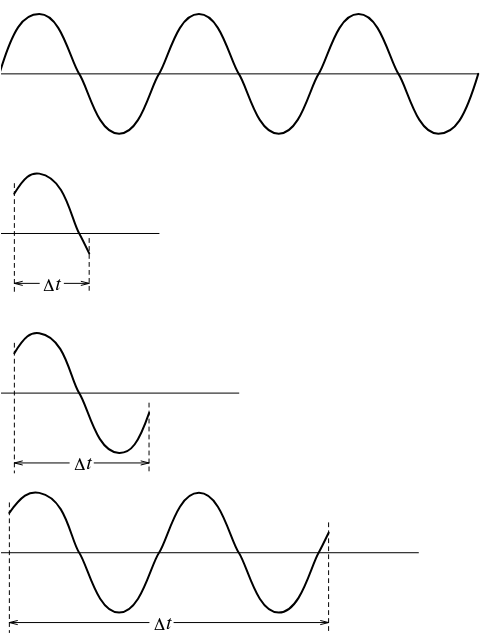
\includegraphics[height=5.5cm]{./gabor2.png}
		\caption{Improved frequency measurement over longer time intervals. The uncertainty in the frequency $\Delta f$ decreases as the measurement interval $\Delta t$ increases and vice versa\footfullcite{gabor2}}
	\end{figure}
\end{frame}

\begin{frame}
	\frametitle{Gabor's Uncertainty Principle, visual}
	\begin{figure}
		\centering
		\subfloat{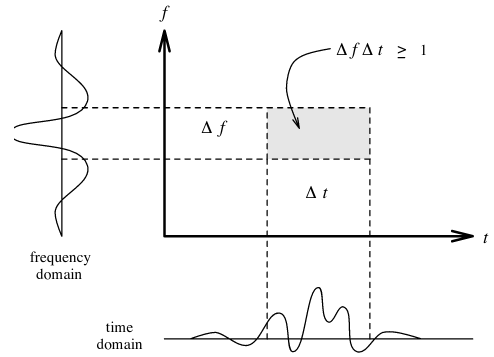
\includegraphics[height=4cm]{./tf-resolution2.png}}
		\hspace{0.35em}
		\subfloat{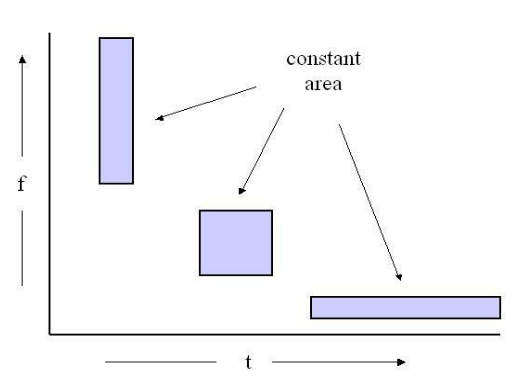
\includegraphics[height=4cm]{./tf-resolution.png}}
		\caption{The most a signal can be localized in the Fourier domain is into rectangles of size $\Delta t\Delta f = 1$}
	\end{figure}
\end{frame}

\begin{frame}
	\frametitle{Consequence of the Fourier transform}
	\begin{quote}
	In time-frequency analysis, it has been proven that linear operators cannot exceed the uncertainty bound [...] Nonlinearity does not by itself confer any acuity advantage, and in fact most nonlinearities are merely distortions and thus deleterious. However, by the above theorem, any carefully crafted analysis that can beat this limit must necessarily be nonlinear.\footfullcite{psycho}
	\end{quote}
\end{frame}

\begin{frame}
	\frametitle{Time-frequency tradeoff, visual}
	Arises from the linearity of the Fourier transform
	\begin{figure}
		\centering
		\subfloat[Unit impulse vs. infinite sine wave\footfullcite{gabor1946}]{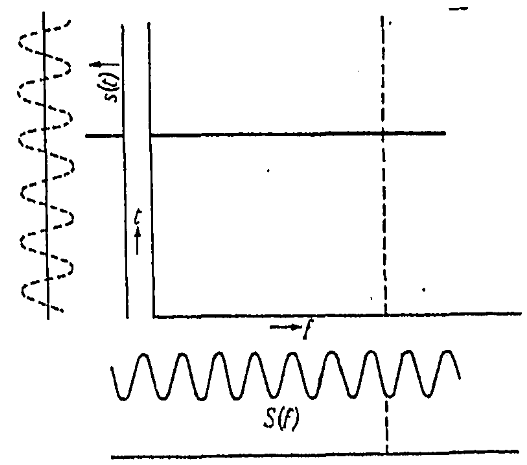
\includegraphics[width=4cm]{./gabor1.png}}
		\hspace{0.2em}
		\subfloat[Spread of a signal and its Fourier transform are inversely proportional\footfullcite{gabor2}]{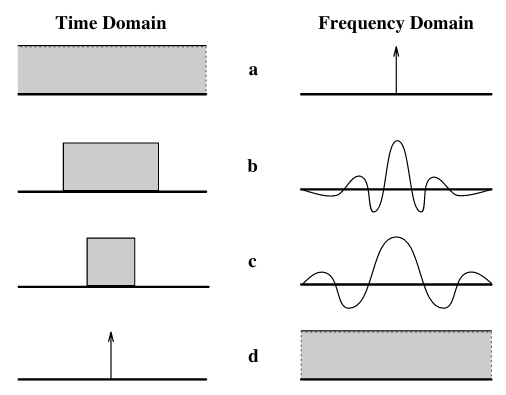
\includegraphics[width=5cm]{./gabor3.png}}
		\caption{Time vs. frequency}
	\end{figure}
\end{frame}

\begin{frame}
	\frametitle{Physical intuitions}
	\begin{quote}
		The foregoing solutions [of the Fourier transform], though unquestionably mathematically correct, are somewhat difficult to reconcile with our physical intuitions and our physical concepts of such variable frequency mechanisms as, for instance, the siren
	\end{quote}
	-- Carson (quoted by Gabor)
	\begin{quote}
	\vspace{2em}
		Gabor came to the conclusion that the difficulty lay in our mutually exclusive formulations of time analysis and frequency analysis ... he suggested a new method of analyzing signals in which time and frequency play symmetrical parts.\footfullcite{korpel}
	\end{quote}
\end{frame}

\note{
	\begin{itemize}
		\item
			this points to the origin of the wavelet and searching for alternative, non-linear representations of time-domain signals
	\end{itemize}
}

\begin{frame}
	\frametitle{Psychoacoustics}
	Psychoacoustic\footfullcite{psycho} studies have shown that humans can exhibit a better time-frequency resolution than Gabor's limit:
	\begin{quote}
		We have conducted the first direct psychoacoustical test of the Fourier uncertainty principle in human hearing, by measuring simultaneous temporal and frequency discrimination. Our data indicate that human subjects often beat the bound prescribed by the uncertainty theorem, by factors in excess of 10.
	\end{quote}
	Similarly to how Gabor was dissatisfied with time-frequency's inability to reconcile with physical intuitions:
	\begin{quote}
		most sound analysis and processing tools today continue to use models based on spectral theories. We believe it is time to revisit this issue.
	\end{quote}
\end{frame}

\note{
	\begin{itemize}
		\item
			In fact its not a defeat of Gabor, its a justification that we need to find better representations -- it actually supports the search for decompositions with non-linear components
	\end{itemize}
}

\begin{frame}
	\frametitle{Psychoacoustics}
	Brian C. J. Moore in 1973:\footfullcite{moore}
	\begin{quote}
		It is concluded that models based on a place (spectral) analysis should be subject to a limitation of the type $\Delta f \dot d \ge \text{constant}$, where $\Delta f$ is the frequency difference limen (DL) for a tone pulse of duration d. [...]  It was found that at short durations the product of $\Delta f$ and d was about one order of magnitude smaller than the minimum predicted from the place model
	\end{quote}
\end{frame}

\note{
	\begin{itemize}
		\item
			frequency difference limen is similar to JND
		\item
			Consider that some psychoacoustic theories of hearing state that the cochlea does a tonotopic spectral decomposition, making it subject to the limitation
	\end{itemize}
}

\begin{frame}
	\frametitle{Gabor elementary functions}
	minimizing area of the tf rectangle
	gaussian-modulated sine waves
	a asymptotic infinity, 0
\end{frame}

\begin{frame}
	\frametitle{Gabor elementary functions}
	show window vs hann
\end{frame}

\begin{frame}
	\frametitle{Gabor elementary functions}
	relation to shannon
\end{frame}

\begin{frame}
	\frametitle{Time-frequency resolution in the STFT}
	Using default MATLAB spectrogram parameters\footfullcite{matlabspecgram} (Hamming window)
	\begin{figure}
		\vspace{-1em}
		\centering
		\subfloat[Good $\Delta t$, bad $\Delta f$]{{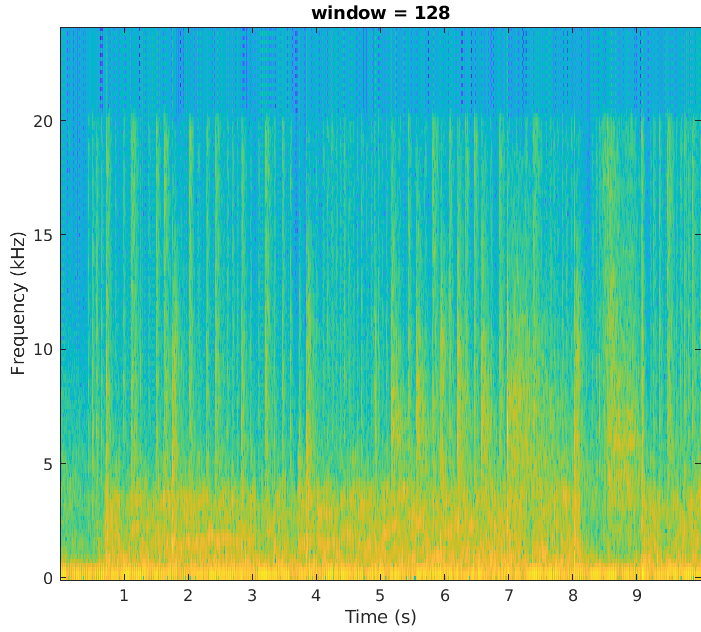
\includegraphics[width=6cm]{./stft_small.png} }}
		\subfloat[Good $\Delta f$, bad $\Delta t$]{{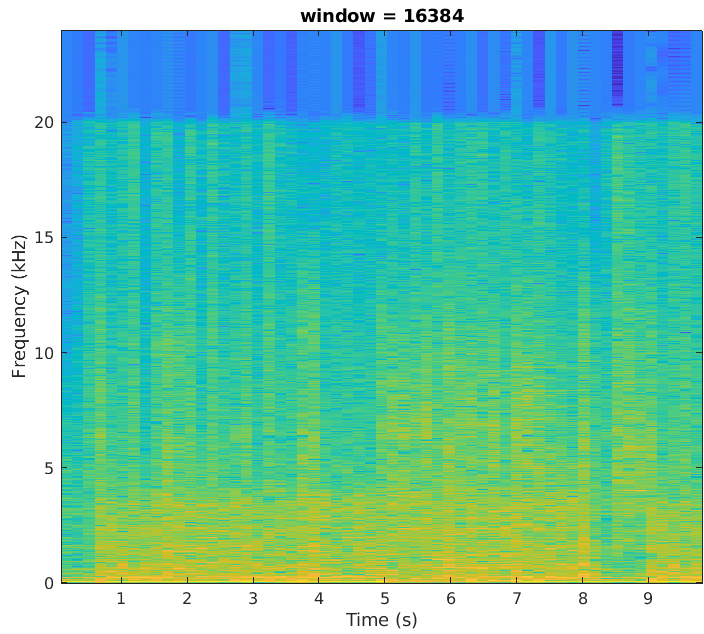
\includegraphics[width=6cm]{./stft_big.png} }}
		\caption{STFT, small vs. big window}
	\end{figure}
\end{frame}

\begin{frame}
	\frametitle{Time-frequency resolution in the STFT}
	\begin{figure}
		\centering
		\subfloat[Good $\Delta t$, bad $\Delta f$]{{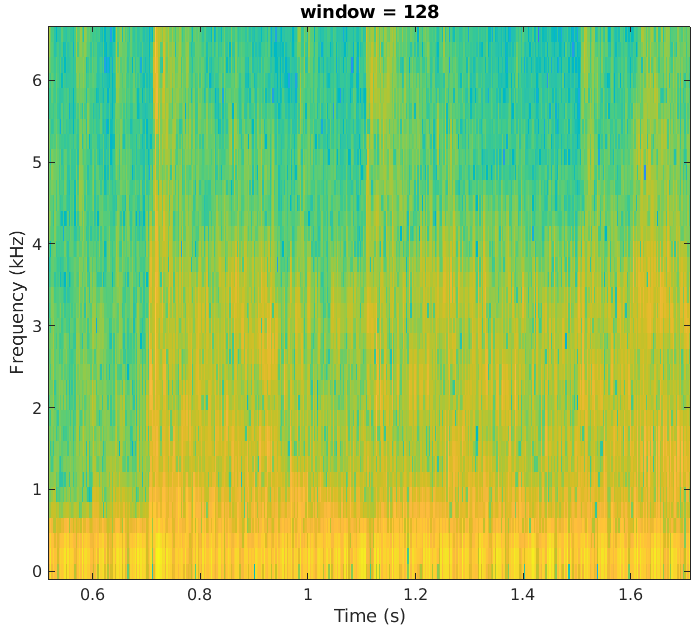
\includegraphics[width=6cm]{./stft_small_zoomed.png} }}
		\subfloat[Good $\Delta f$, bad $\Delta t$]{{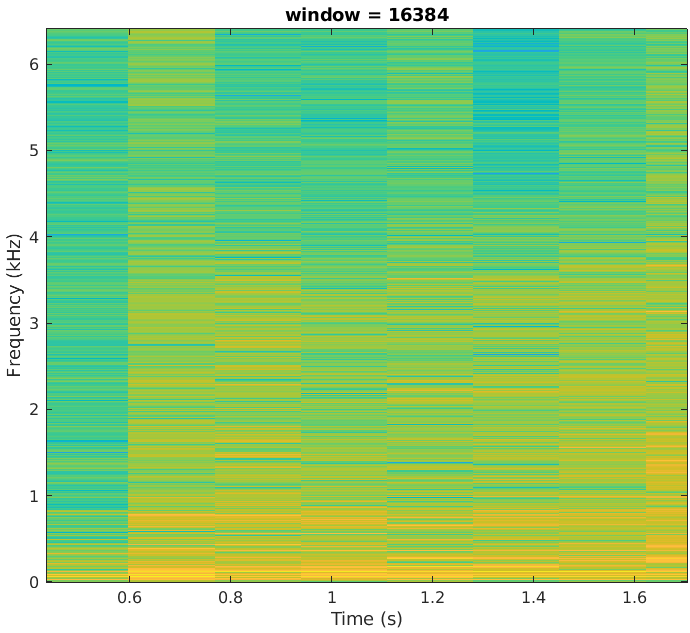
\includegraphics[width=6cm]{./stft_big_zoomed.png} }}
		\caption{STFT, small vs. big window}
	\end{figure}
\end{frame}

\begin{frame}
	\frametitle{Gabor transform -- best possible TF resolution}
\end{frame}

\begin{frame}
	\frametitle{Problems with Gabor}
	non-orthogonal? infinite gaussian?
\end{frame}

\end{document}
